\documentclass{beamer}

\usepackage{graphicx}
\usepackage{amssymb}% http://ctan.org/pkg/amssymb
\usepackage{pifont}% http://ctan.org/pkg/pifont
\newcommand{\cmark}{\ding{51}}%
\newcommand{\xmark}{\ding{55}}%

\title{Types in HorseIR}
\author{Hongji Chen}
\date{August 3, 2017}

\usecolortheme{seagull}
\useoutertheme{infolines}
\usefonttheme[onlymath]{serif}

\begin{document}
    
\maketitle

\begin{frame}
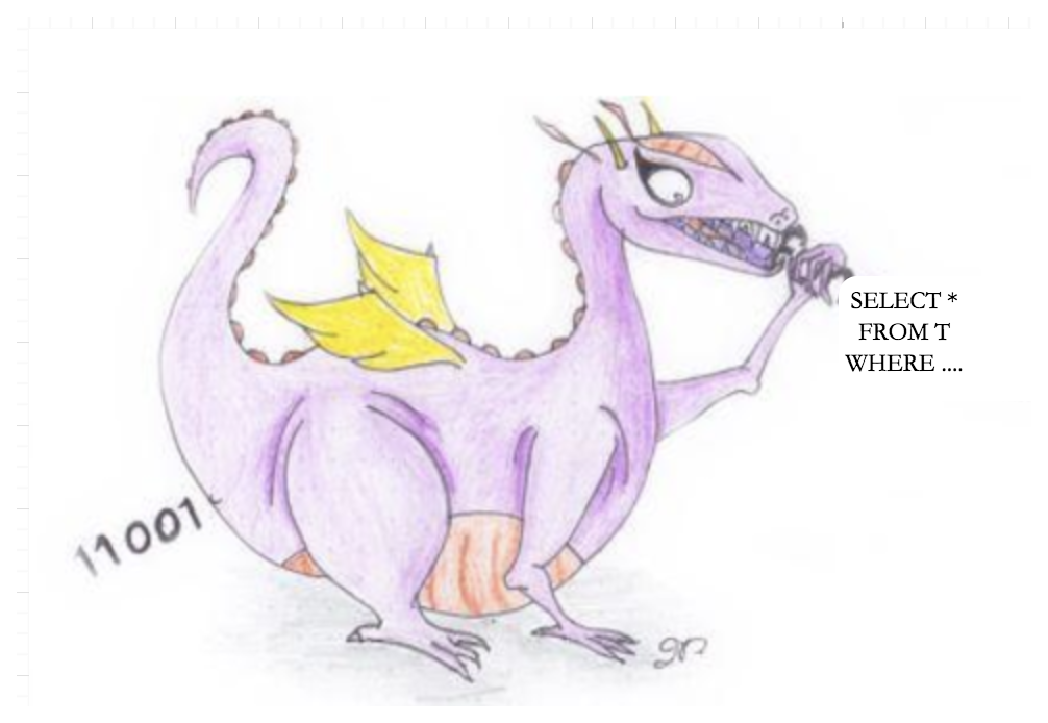
\includegraphics[width=\textwidth]{logo-dragon}
\end{frame}

\begin{frame}{Overview}
\begin{itemize}
    \item \textbf{ScalarType}: 
          integers, floating point numbers, characters, $\dots$
    \item \textbf{WildcardType}: 
          anything (defer to runtime)
    \item \textbf{list$\langle$T$\rangle$}: 
          a list with $T$-typed elements
    \item \textbf{dict$\langle$K, V$\rangle$}: 
          a list with $K$-typed keys and $V$-typed values
    \item \textbf{enum$\langle$T$\rangle$}: 
          a enumeration with $T$-typed elements
    \item \textbf{func$\langle$T1, T2, T3, $\dots$ $:$R$\rangle$}: 
          a function with $T1$-typed first argument, $T2$-typed second
          argument, $T3$-typed third argument and $R$-typed return argument
\end{itemize}
\end{frame}

\begin{frame}{Type Conversion}
\begin{itemize}
    \item \textbf{Trivial Conversion}: no memory r/w required, guaranteed safe
          at runtime, and check at compile time (e.g. $i32 \rightarrow ?)$
    \item \textbf{Casting}: memory r/w may required (e.g. $i32 \rightarrow
          i64$)
    \item \textbf{Runtime Conversion}: required runtime checking (e.g. $?
          \rightarrow i32$)
          \begin{itemize}
          \item \textbf{check\_cast(x, T)}: \\ query runtime information about
                $x$ and cast to type $T$ if necessary
          \item \textbf{check\_type(x, T)}: \\ determine whether $x$ has type
                $T$ and return query result as a boolean value
          \end{itemize}
\end{itemize}
\end{frame}

\begin{frame}{Trivial Conversion}
\begin{block}{$T1$.isGeneralizationOf($T2$)}
\begin{itemize}
    \item if $T1$ is scalar type, then $T1$.isGeneralizationOf($T2$)
          $\iff$ $T2$ is also a scalar and has the same scalar type,
    \item if $T1$ is wildcard type, then $T1$.isGeneralizationOf($T2$)
          is also true,
    \item if $T1$ is list$\langle E1 \rangle$, then
          $T1$.isGeneralizationOf($T2$) $\iff$ $T2$ has type
          list$\langle E2 \rangle$ with $E1$.isGeneralizationOf($E2$),
    \item if $T1$ is dict$\langle K1,V1 \rangle$, then 
          $T1$.isGeneralizationOf($T2$) $\iff$ $T2$ has type
          dict$\langle K2, V2 \rangle$ with $K1$.isGeneralizationOf($K2$)
          $\land$ $V1$.isGeneralizationOf($V2$),
    \item if $T1$ is enum$\langle E1 \rangle$, then
          $T1$.isGeneralizationOf($T2$) $\iff$ $T2$ has type
          enum$\langle E2 \rangle$ with $E1$.isGeneralizationOf($E2$),
    \item if $T1$ is func$\langle E1_1, E1_2, \dots :R1 \rangle$, then 
          $T1$.isGeneralizationOf($T2$) $\iff$ $T2$ has type 
          func$\langle E2_1, E2_2, \dots :R2 \rangle$, with $\forall i$, 
          $E1_i$.isGeneralizationOf($E2_i$) $\land$ 
          $R1$.isGeneralizationOf($R2$)
\end{itemize}
\end{block}
\end{frame}

\begin{frame}[fragile]{$T1$.isGeneralizationOf($T2$)}
\begin{block}{Examples}
\begin{enumerate}
    \item $T1 : i32$, and $T2 : i64$ $\Rightarrow$ 
          $T1$.isGeneralizationOf($T2$) \xmark
    \item $T1 : i32$, and $T2 : i32$ $\Rightarrow$
          $T1$.isGeneralizationOf($T2$) \cmark
    \item $T1 : \text{dict}\langle \text{list}\langle ? \rangle, \text{bool}
          \rangle$, and $\text{dict}\langle \text{list}\langle i32 \rangle,
          \text{bool} \rangle$ $\Rightarrow$ $T1$.isGeneralizationOf($T2$)
          \cmark
    \item $T1 : \text{dict}\langle \text{list}\langle ? \rangle, \text{bool}
          \rangle$, and $\text{dict}\langle \text{list}\langle i32 \rangle,
          ? \rangle$ $\Rightarrow$ $T1$.isGeneralizationOf($T2$) \xmark
    \item $T1 : \text{func}\langle i32, ... : ?\rangle \rightarrow
                \text{func}\langle i32, ?, ? : ?\rangle$, and
          $T2 : \text{func}\langle i32, \text{bool}, \text{char} : ? \rangle$
          $\Rightarrow$ $T1$.isGeneralizationOf($T2$) \cmark
\end{enumerate}    
\end{block}
\end{frame}

\begin{frame}{Overloading in HorseIR}
\begin{itemize}
    \item To select the best implementation for primitive functions based on
          types information.
    \item for method call with signature type $T$, and candidate methods $T_1,
          T_2, T_3, \dots$, select $T_k$ such that,
          \begin{itemize}
          \item $T_k$.isGeneralizationOf($T$)
          \item $\forall i \neq k$, $\neg$ $T_k$.isGeneralizationOf($T_i$)
          \end{itemize}
\end{itemize}
\end{frame}

\begin{frame}{Overloading in HorseIR - Examples}
\begin{block}{Candidate methods}
\begin{itemize}
    \item $\text{add1} : \text{func}\langle ... : ? \rangle $,
    \item $\text{add2} : \text{func}\langle ?, ? : ? \rangle$,
    \item $\text{add3} : \text{func}\langle \text{list} \langle ? \rangle,
           \text{list} \langle ? \rangle : \text{list} \langle ? \rangle
           \rangle$,
    \item $\text{add4} : \text{func}\langle \text{list} \langle i32 \rangle,
           \text{list} \langle i32 \rangle : \text{list} \langle i32 \rangle
           \rangle$.
\end{itemize}
\end{block}
\begin{itemize}
    \item $(i32)$ $\Rightarrow$ add1
    \item $(i32, i32)$ $\Rightarrow$ add2
    \item $(\text{list} \langle f32 \rangle, \text{list} \langle f64 \rangle)$
          $\Rightarrow$ add3
    \item $(\text{list} \langle i32 \rangle, \text{list} \langle i64 \rangle)$
          $\Rightarrow$ add3
    \item $(\text{list} \langle i32 \rangle, \text{list} \langle i32 \rangle)$
          $\Rightarrow$ add4
\end{itemize}
\end{frame}

\begin{frame}{Overloading in HorseIR - Ambiguity} 
\begin{block}{Candidate methods}
\begin{itemize}
    \item $foo1 : \text{func}\langle i32, ? : \text{bool} \rangle$,
    \item $foo2 : \text{func}\langle ?, i32 : \text{bool} \rangle$.
\end{itemize}
\end{block}  
with invoking parameter types $(i32, i32)$, choose which method?

$\Rightarrow$ Ambiguity
\end{frame}

\begin{frame}{Specificity Join}
\begin{itemize}
    \item aim to remove ambiguity during dispatch process,
    \item attempt to create a type pattern representing the intersection
          between two type matched sets,
          \begin{center}
              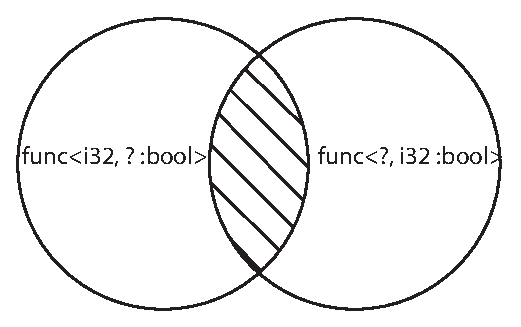
\includegraphics{Fig_Intersection}
          \end{center}
\end{itemize}
\end{frame}

\begin{frame}{Specificity Join}
\begin{itemize}
    \item rule-based join
    \item traverse both AST tree at same time, on each node, select the node
          containing more information about matched type 
\end{itemize}
\end{frame}

\begin{frame}{Specificity Join}
\centering
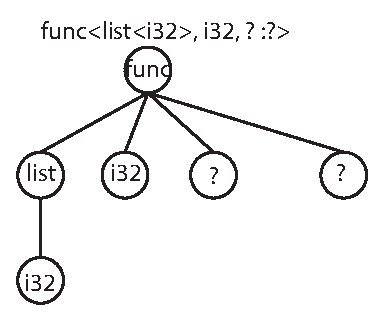
\includegraphics{Fig_Type1}
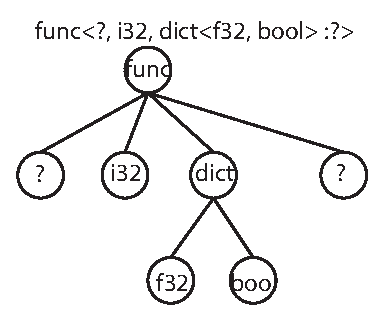
\includegraphics{Fig_Type2}
\end{frame}

\begin{frame}{Specificity Join}
\centering
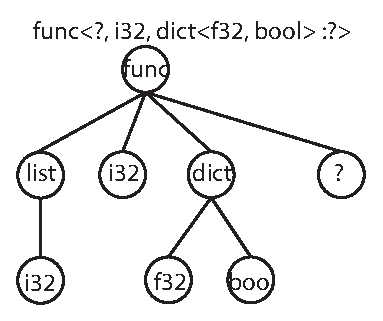
\includegraphics{Fig_TypeJoin}
\end{frame}

\begin{frame}{Specificity Join}
\begin{itemize}
    \item attempt to create $T_{join}$ for $T_1$ and $T_2$,
    \item if $T_{join}$ not exists $\Rightarrow$ claim no intersection
          between $T_1$ and $T_2$,
    \item test $T_1$.isGeneralizationOf($T_{join}$) $\land$ 
               $T_2$.isGeneralizationOf($T_{join}$) 
          \begin{itemize}
          \item T $\Rightarrow$ ambiguity exists,
          \item F $\Rightarrow$ no intersection between $T_1$ and $T_2$.
          \end{itemize}
\end{itemize}
\end{frame}

\begin{frame}{Specificity Join}
\begin{itemize}
    \item $T_1 : \text{func}\langle i32, ? : ? \rangle$
    \item $T_2 : \text{func}\langle ?, i32 : ? \rangle$
    \item $T_{join} = \text{specificityJoin}(T_1, T_2)
                    = \text{func}\langle i32, i32 : ? \rangle$
    \item $T_1$.isGeneralizationOf($T_{join}$) \cmark, and 
          $T_2$.isGeneralizationOf($T_{join}$) \cmark
    \item \textbf{Ambiguity Exists} 
\end{itemize}
\end{frame}

\begin{frame}{Overload in HorseIR - Summary}
\begin{block}{Building overloading candidate pool}
add method $M$ with signature type $T$ into candidate pool containing existed
overloading option with type $T_1, T_2, T_3, \dots$.
\begin{itemize}
    \item $\forall i$, construct $T_i^{join} :=$ specificityJoin$(T, T_i)$
    \item if $T_i^{join}$ not exist, add $M$ to pool
    \item test $T$.isGeneralizationOf($T_i^{join}$) $\land$
               $T_i$.isGeneralizationOf($T_i^{join}$)
          \begin{itemize}
          \item T $\Rightarrow$ raise error
          \item F $\Rightarrow$ add $M$ to pool
          \end{itemize}
\end{itemize}
\end{block}
\textbf{Unique Overloading Option Property} \\
$\forall T,i,j$ \\
$T_i$.isGeneralizationOf($T$) $\land$  
($\forall z\neq i \quad \neg T_i$.isGeneralizationOf($T_z$)) $\land$ \\
$T_j$.isGeneralizationOf($T$) $\land$  
($\forall z\neq j \quad \neg T_j$.isGeneralizationOf($T_z$))         \\
$\rightarrow i = j$
\end{frame}

\begin{frame}{Implementation in HorseIR project}
\begin{itemize}
    \item under namespace horseIR::interpreter::VectorDispatcher
    \item \textbf{manage} add a overloading option, with given package name, 
          method name, and signature
    \item \textbf{fetch} dispatch a method call with given package name, method
          name and input parameter types
\end{itemize}
\end{frame}

\begin{frame}{Demo}
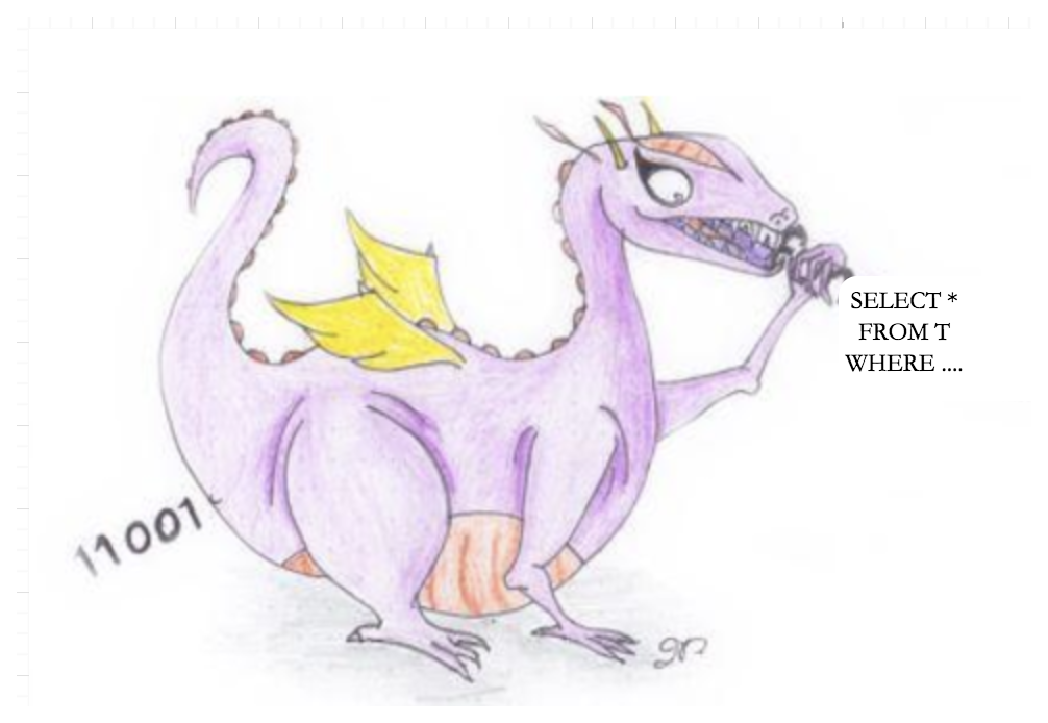
\includegraphics[width=\textwidth]{logo-dragon}
\end{frame}

\end{document}
